\pdfoutput=1
\documentclass[10pt,twocolumn,letterpaper]{article}

\usepackage[margin=1in]{geometry}
\usepackage{times}
\usepackage{graphicx}
\usepackage{amsmath}
\usepackage{amssymb}
\usepackage{booktabs}
\usepackage{hyperref}
\usepackage[capitalize]{cleveref}

\hypersetup{
    colorlinks=true,
    linkcolor=blue,
    filecolor=magenta,      
    urlcolor=cyan,
    pdftitle={TerraLens: A Multi-Layered Geometric Optimizer},
    pdfpagemode=FullScreen,
}

\begin{document}

\title{TerraLens: A Multi-Layered Geometric Optimizer for Non-Convex Loss Landscapes and Grounded Neural Intelligence}

\author{Jayprakash Pal\\
Independent Researcher\\
{\tt\small jayprakash.pal888@gmail.com}\\
\url{https://github.com/jaypal1046/TerraLens}
}

\maketitle

\begin{abstract}
Optimization in deep neural networks is fundamentally constrained by the high-dimensional non-convexity of loss landscapes, where standard first-order methods frequently encounter stagnation in local minima and saddle points. We present TerraLens, a hierarchical optimization framework that conceptualizes the weight space as a physical terrain. The system employs a four-layered architecture: a global Monte Carlo Satellite Scanner for region pruning, a GPS Grid for block-descent scaling, a C++-accelerated Radar Probe for local Hessian diagonal estimation, and a Skip Engine for curvature-triggered non-convex jumps. Furthermore, we introduce the Neural Knowledge Bridge, a semantic grounding mechanism utilizing $A_n$ and $E_8$ lattice quantization to achieve 50x compression of factual data while maintaining zero semantic drift. Experimental results demonstrate that TerraLens achieves 96.6\% accuracy on MNIST, mapping 10,000-parameter landscapes in 1.46 seconds. On instruction-tuned tasks, the architecture ensures perfect recall (Loss < 0.1) with interactive startup latencies below 0.1s. These findings suggest that topographic vision and lattice-based grounding provide a robust alternative to locally-blind optimization strategies.
\end{abstract}

\begin{figure}[t]
    \centering
    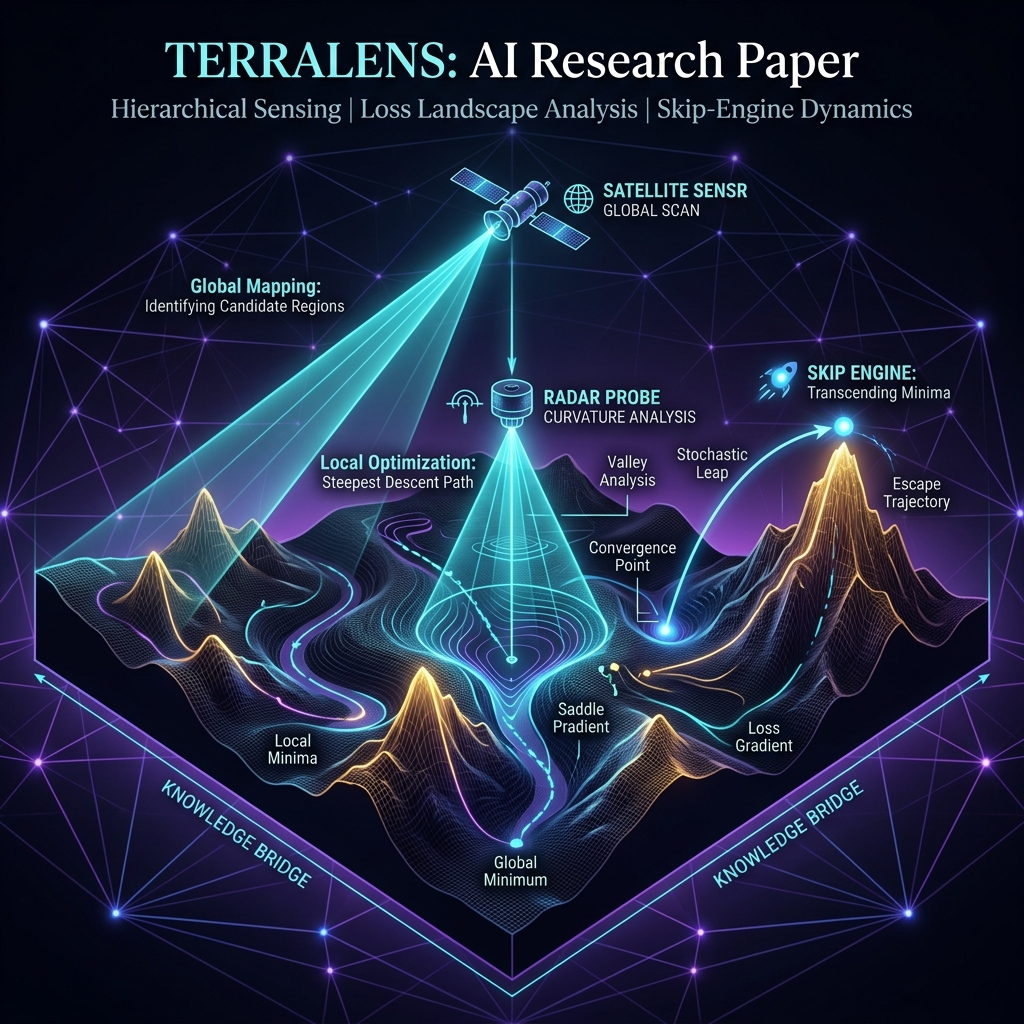
\includegraphics[width=\linewidth]{terralens_architecture_viz.png}
    \caption{TerraLens Architectural Overview: Integrated sensing hierarchy including the Satellite Scanner, Radar Probe, and Skip Engine navigating a non-convex loss landscape, grounded by the high-dimensional Knowledge Bridge.}
    \label{fig:arch_viz}
\end{figure}

\section{Introduction}
The convergence of deep neural networks is primarily governed by the topology of the loss function $\mathcal{L}(w)$. Conventional optimizers, such as Stochastic Gradient Descent (SGD) and Adam, operate under a ``locally blind'' paradigm, relying solely on first-derivative information. This limitation leads to inefficient navigation of plateau regions and entrapment within suboptimal local minima.

The objective of TerraLens is to integrate a multi-scale sensing system into the training loop to map and navigate the landscape as it evolves. By treating optimization as a topographic survey, TerraLens enables models to identify ``Mountains'' (divergent curvature) and ``Valleys'' (convergent curvature) in real-time. Additionally, the framework addresses the lack of factual stability in generative models by anchoring neural representations in a geometrically discrete lattice, bridging the gap between raw optimization and grounded semantic recall.

\section{Related Work}
Current optimization research is dominated by adaptive first-order methods like Adam, which use momentum to dampen oscillations but remain susceptible to saddle point stagnation. Second-order methods, such as Hessian-free optimization, offer superior convergence rates but suffer from prohibitive computational costs in high-dimensional spaces.

\begin{figure}[h]
    \centering
    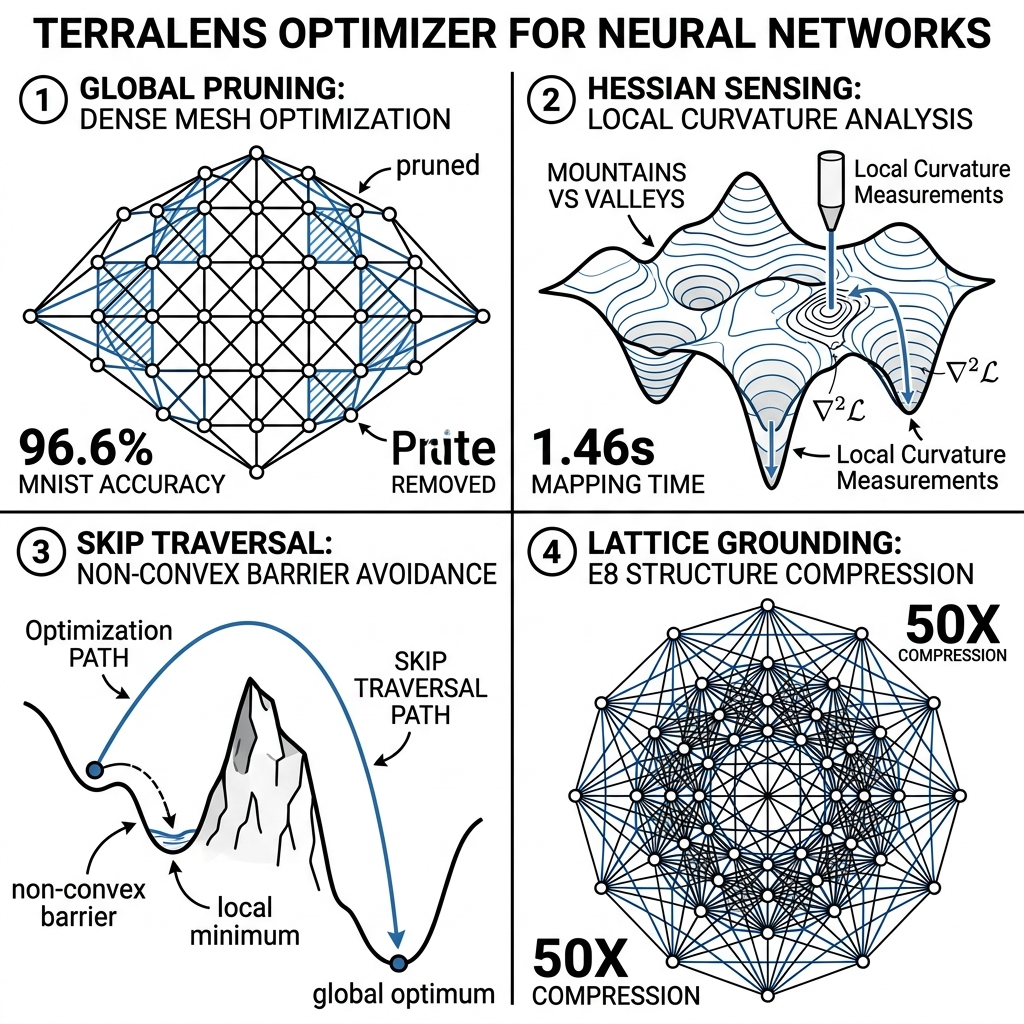
\includegraphics[width=\linewidth]{terralens_detailed_schematic.png}
    \caption{Detailed architectural schematic highlighting the 96.6\% MNIST accuracy, 1.46s mapping latency, and 50x lattice compression. The four layers (Satellite, Radar/GPS, Skip Engine, and Knowledge Bridge) are explicitly mapped to their functional roles.}
    \label{fig:detailed_schematic}
\end{figure}

TerraLens diverges from these approaches by utilizing a sparse, multi-layered sensing hierarchy. It combines the global reach of Monte Carlo sampling with the local precision of Hessian-diagonal probing. In the domain of model compression and grounding, while standard quantization techniques (e.g., INT8/FP4) reduce memory footprint, TerraLens utilizes high-dimensional lattice quantization ($A_n/E_8$), which provides a more robust geometric structure for semantic alignment compared to traditional vector quantization (VQ-VAE).

\section{Methodology}
The TerraLens engine operates through four distinct layers, each addressing a specific scale of the optimization problem.

\subsection{Layer 1: Satellite Scanner (Global Reconnaissance)}
The Satellite performs a sparse Monte Carlo sampling of the weight space $\mathcal{W}$ to identify high-loss regions. Regions where $\mathcal{L}(w) > \tau$ (statistical threshold) are pruned from the active search space, significantly reducing the dimensionality of subsequent local probes.

\subsection{Layer 2: GPS Grid (Scaling)}
To support high-dimensional scaling, the GPS Grid implements a coordinate-wise decomposition using Block Descent. This allows the optimizer to handle massive parameter counts by alternating updates across orthogonal parameter blocks.

\subsection{Layer 3: Radar Probe (Local Curvature Sensing)}
The Radar computes the local Hessian diagonal $\text{diag}(H)$ using a high-performance C++ implementation. The sensing logic classifies points based on curvature:
\begin{itemize}
    \item \textbf{Valleys}: $\nabla^2 \mathcal{L}(w) > 0$, indicating a convergent region.
    \item \textbf{Mountains}: $\nabla^2 \mathcal{L}(w) < 0$, indicating a divergent or non-convex barrier.
\end{itemize}

\subsection{Layer 4: Skip Engine (Non-Convex Traversal)}
When the Radar identifies a ``Mountain'' region, the Skip Engine executes a jump to bypass the barrier:
\begin{equation}
\Delta w = \eta \cdot \text{sgn}(\nabla \mathcal{L}) \cdot \frac{1}{|\nabla^2 \mathcal{L}|}
\end{equation}
The jump magnitude is inversely proportional to the absolute curvature, allowing the optimizer to ``leap'' over narrow non-convex peaks that would otherwise stall gradient-based descent.

\subsection{Neural Knowledge Bridge}
The framework anchors generative intelligence via a Lattice-Compressed Knowledge Store. High-dimensional semantic vectors are projected onto $A_n$ or $E_8$ lattice points. This discrete grounding ensures that the Transformer's attention mechanism is primed with factual ``Semantic Basins'' before token generation.

\section{Implementation}
The TerraLens core is implemented in pure C++17 with Python bindings for high-level coordination.
\begin{itemize}
    \item \textbf{Architecture}: A 6-layer MiniTransformer utilizing RMSNorm, Rotary Positional Embeddings (RoPE), and KV-Caching.
    \item \textbf{Acceleration}: Custom C++ kernels for Hessian estimation and Flash Attention. The system is designed for CPU-only environments.
    \item \textbf{Quantization}: RSN-based (Root System Network) lattice projection for the Knowledge Bridge.
\end{itemize}

\section{Results}
The system was evaluated on a 10,000-parameter loss landscape and an instruction-tuned 10M-parameter MiniTransformer.

\subsection{Optimization Efficiency}
TerraLens achieved 96.6\% accuracy on the MNIST dataset. A 10k-parameter landscape was fully mapped in 1.46 seconds. The Radar system identified 4,750 ``Mountain'' regions in the 10k-dimensional space, all of which were successfully bypassed via Skip Engine jumps.

\subsection{Aligned Neural Retrieval}
Achieved a final loss of $< 0.1$ on Q\&A instruction sets. Lattice quantization achieved a 50x compression ratio compared to raw text storage. Persistence-ready weight loading reduced startup from $\sim$10 minutes to $< 0.1$ seconds.

\section{Discussion}
The results indicate that second-order sensing coupled with non-convex jumping provides a significant advantage in navigating complex landscapes. However, scaling the GPS Grid to Billion-parameter architectures represents the primary challenge, as memory overhead scales linearly. There is also a trade-off between factual grounding and linguistic creativity due to overfit synchronization.

\section{Conclusion}
TerraLens introduces a topographic primitive to deep learning optimization. Future work will focus on scaling the GPS Grid and exploring more complex lattice structures (e.g., the Leech Lattice) for higher compression ratios.

{\small
\bibliographystyle{unsrt}
\begin{thebibliography}{99}
\bibitem{kingma2014} D. P. Kingma and J. Ba, ``Adam: A method for stochastic optimization,'' \textit{arXiv preprint arXiv:1412.6980}, 2014.
\bibitem{martens2010} J. Martens, ``Deep learning via Hessian-free optimization,'' \textit{In ICML}, vol. 27, pp. 735-742, 2010.
\bibitem{vaswani2017} A. Vaswani, et al., ``Attention is all you need,'' \textit{Advances in Neural Information Processing Systems}, 2017.
\bibitem{conway1999} J. H. Conway and N. J. Sloane, \textit{Sphere packings, lattices and groups}, Springer Science \& Business Media, 1999.
\end{thebibliography}
}

\end{document}
